%% 
%% Copyright 2007, 2008, 2009 Elsevier Ltd
%% 
%% This file is part of the 'Elsarticle Bundle'.
%% ---------------------------------------------
%% 
%% It may be distributed under the conditions of the LaTeX Project Public
%% License, either version 1.2 of this license or (at your option) any
%% later version.  The latest version of this license is in
%%    http://www.latex-project.org/lppl.txt
%% and version 1.2 or later is part of all distributions of LaTeX
%% version 1999/12/01 or later.
%% 
%% The list of all files belonging to the 'Elsarticle Bundle' is
%% given in the file `manifest.txt'.
%% 
%% Template article for Elsevier's document class `elsarticle'
%% with harvard style bibliographic references
%% SP 2008/03/01

%\documentclass[preprint,12pt,authoryear]{elsarticle}  %default in the template
%\documentclass[preprint,10pt,authoryear]{elsarticle}

%% Use the option review to obtain double line spacing
%% \documentclass[authoryear,preprint,review,12pt]{elsarticle}

%% Use the options 1p,twocolumn; 3p; 3p,twocolumn; 5p; or 5p,twocolumn
%% for a journal layout:
% \documentclass[final,1p,times,authoryear]{elsarticle}
%% \documentclass[final,1p,times,twocolumn,authoryear]{elsarticle}
 \documentclass[final,3p,times,authoryear]{elsarticle}
%% \documentclass[final,3p,times,twocolumn,authoryear]{elsarticle}
%% \documentclass[final,5p,times,authoryear]{elsarticle}
%% \documentclass[final,5p,times,twocolumn,authoryear]{elsarticle}

%% For including figures, graphicx.sty has been loaded in
%% elsarticle.cls. If you prefer to use the old commands
%% please give \usepackage{epsfig}

%% The amssymb package provides various useful mathematical symbols
\usepackage{amssymb}
%% The amsthm package provides extended theorem environments
\usepackage{amsthm}
\usepackage{amsmath}
\usepackage{color, colortbl}
\usepackage{amsmath}
\usepackage{siunitx}
\usepackage{tabularx}
\usepackage[]{algorithm2e}
\usepackage{soul}
\usepackage{glossaries}
\usepackage{subfig}
\usepackage{scalerel}
\usepackage{ulem}

%track changes on
%\newcommand{\add}[1]{\textcolor{blue}{#1}}
%\newcommand{\remove}[1]{\textcolor{red}{\st{#1}}}
%track changes off
\newcommand{\add}[1]{\textcolor{black}{#1}}
\newcommand{\remove}[1]{\textcolor{red}{\st{}}}


\definecolor{light-gray}{gray}{0.9}


\newcommand{\beginsupplement}{%
        \setcounter{table}{0}
        \renewcommand{\thetable}{S\arabic{table}}%
        \setcounter{figure}{0}
        \renewcommand{\thefigure}{S\arabic{figure}}%
     }


\DeclareRobustCommand{\hlgreen}[1]{{\sethlcolor{green}\hl{#1}}}

\journal{Building and Environment}
\makeglossaries


\begin{document}


\title{Isolating the impacts of urban form and fabric from geography on urban heat and human thermal comfort}

\author[melb]{Kerry~A.~Nice\corref{cor1}}
\cortext[cor1]{Principal corresponding author}
\ead{kerry.nice@unimelb.edu.au}
\author[arc,built]{Negin Nazarian}
\author[arc]{Mathew J. Lipson}
\author[arc]{Melissa A. Hart}
\author[melb]{Sachith Seneviratne}
\author[melb]{Jason Thompson}
\author[arc]{Marzie Naserikia}
\author[melb]{Branislava Godic}
\author[melb,eng]{Mark Stevenson}
\address[melb]{Transport, Health, and Urban Design Research Lab, Faculty of Architecture, Building, and Planning, University of Melbourne, VIC, Australia.}
\address[arc]{ARC Centre of Excellence for Climate Extremes, University of New South Wales, Sydney, NSW, Australia.}
\address[built]{School of Built Environment; and City Futures Research Centre, University of New South Wales, Sydney, NSW, Australia.}
\address[eng]{Melbourne School of Engineering; and Melbourne School of Population and Global Health, University of Melbourne, VIC, Australia.}




\begin{abstract}


\remove{As public}\add{Public} health risks resulting from urban heat in cities \remove{increase}\add{are increasing} due to \add{rapid} urbanisation and climate change, \remove{there is a pressing need}\add{motivating closer attention} to\remove{design strategies for} urban heat mitigation and \remove{ensure}\add{adaptation strategies} that\remove{future development is climate sensitive. Heat} \add{enable  climate-sensitive urban design and development. These strategies incorporate four key factors influencing heat} stress in \remove{cities is mainly influenced by four factors:}\add{cities:} the urban form (morphology of vegetated and built surfaces), urban fabric, urban function (including human activities), and background climate and regional geographic settings (e.g. topography and distance to water bodies). The first two factors can be modified and redesigned as urban heat mitigation strategies (e.g. changing the albedo of surfaces, replacing hard surfaces with pervious vegetated surfaces, or increasing canopy \remove{cover), whereas}\add{cover). Regional geographical settings of cities, on the other hand, cannot be modified and} while human activities can be modified, \add{it often requires holistic behavioural and policy modifications and} the impacts of these can be difficult to \remove{quantify, and regional geographical settings of cities cannot be modified. However, when}\add{quantify. When} evaluating the effectiveness of urban heat mitigation strategies \add{in observational or traditional modelling studies}\remove{based on modifications to the built and natural forms}, it can be difficult to separate \remove{their}\add{the} impacts \add{of modifications to the built and natural forms} from the interactions of the geographic influences\add{, limiting the universality of results}. \add{To address this, we introduce a new methodology to determine the influence of urban form and fabric on thermal comfort, by utilising a comprehensive combination of possible urban forms, an urban morphology data source, and micro-climate modelling.} \add{We perform 9814 simulations} covering \remove{the full}\add{a wide} range of realistic built and natural forms \remove{(building density and height,}\add{(building,} roads, grass, and tree \remove{density}\add{densities as well as building} and\remove{height)} \add{tree heights)}\remove{in cities, along with a combination of mitigation strategies,} to determine \remove{the}\add{their} importance and influence \remove{of each}on thermal \remove{performance.}\add{environments in urban canyons without geographical influences.} We show that \remove{during the daytime,}higher \add{daytime} air temperatures and \remove{Universal Thermal Climate Index temperatures}\add{thermal comfort indices} are strongly driven by increased street fractions, with \add{maximum} air temperatures \remove{increasing}\add{increases of} up to 10 and 15$^{\circ}$C as street fractions increase \add{from 10\% (very narrow street canyons and/or extensive vegetation cover)} to 80 and \remove{90\%. Reductions}\add{90\% (wide street canyons). Up to 5$^{\circ}$C reductions} in \add{daytime} air \remove{temperature of 5$^{\circ}$C}\add{temperatures} are seen with increasing grass and tree fractions from \remove{none}\add{zero (fully urban)} to complete \add{(fully natural)} coverage. Similar patterns are seen with the Universal Thermal Climate \remove{Index,}\add{Index (UTCI),} with increasing street fractions of 80\% and 90\% driving increases of 6 and \remove{12$^{\circ}$C.}\add{12$^{\circ}$C, respectively.} We then \remove{scale up}\add{apply} the results \remove{to produce}\add{at a} city-wide \add{scale, generating} heat maps of several Australian cities showing the \remove{impact}\add{impacts} of present day urban \remove{form.}\add{form and fabric.} The resulting method allows mitigation strategies to be tested on modifiable urban form factors isolated from geography, topography, and local weather conditions, factors that cannot easily be modified.

\end{abstract}

\begin{keyword}
micro-climate modelling\sep 
urban morphology\sep
heat mitigation\sep
urban heat
\end{keyword}



\maketitle

\section{Introduction}

\subsection{Need for urban heat mitigation measures}

Measures of cumulative heat show significant increases in recent decades with trends of increased heatwave frequency and duration seen globally \citep{Perkins-Kirkpatrick2020}. Exposure to dangerous levels of heat stress \remove{are expected to}\add{may} increase by a factor of 5-10 by 2080 \citep{Coffel2018}, driven by more frequent, severe, and long-lasting heatwaves \citep{IPCC2022}. Heat \remove{in urban areas}is the most dangerous natural hazard in \add{many places in the world, including} Australia \citep{Coates2014} and Europe \citep{Forzieri2017}, with disproportionate risks falling on vulnerable populations such as elderly and the very young \citep{Nicholls2008}. 

The design of cities has \remove{enhanced these}\add{exacerbated the} risks \remove{by replacing}\add{associated with heat extremes. Urbanisation replaces} natural pervious land covers with hard \remove{heat absorbent}\add{heat-absorbent} surfaces, \remove{resulting in increased heat stress for inhabitants. This urbanisation of land-use has altered}\add{altering} the \remove{urban}\add{surface} energy balance \add{in cities} \citep{Oke1982}. Anthropogenic waste heat from buildings and transport \add{as well as shadowing} and \remove{reduced shading through diminishing tree}\add{radiation trapping within the urban} canopy \remove{cover}result in larger amounts of net energy at street level. Meanwhile, the conversion of vegetated to impervious surfaces, and the reduction of available water in cities, shifts the urban energy balance away from latent heat (water evaporation) towards increased sensible heat (heat that can be felt) and increased heat storage in urban surfaces. \remove{Mitigation strategies that incorporate findings from urban climate research into planning}\add{Collectively, the modification} of \remove{future developments can ensure that newly}\add{the urban energy balance result in higher canopy air and surface temperatures in the} built \remove{areas}\add{environments compared to natural land covers, exacerbating heat stress risks for inhabitants} \citep{Coutts2012,Martilli2020}. 

\add{Reviewing the influence of cities on local meteorology, urban climates} are \add{influenced by four key factors: 1) urban form (morphology of vegetated and built surfaces), 2) urban fabric (built materials as well as the natural and vegetated cover, i.e., soil, water, vegetation and their phenology), 3) urban functions (influencing emissions of heat, moisture and pollutants released by human activities), and 4) background} climate\remove{sensitive} and \remove{better able}\add{regional geography \citep{Masson2020a,mills2021characterising}. Urban heat mitigation strategies consider a combination of these factors in planning and design of urban developments, aiming} to address the adverse effects of urban design on the thermal environment. These strategies, which \add{often} rely on modifications to \remove{built form, fabric,}\add{urban form} and \remove{natural land cover}\add{fabric} in cities, require both an understanding of the processes driving excess heat, and the methods required to identify the existing areas of high risk that will benefit most from interventions. \remove{, in}\add{In} a systematic \remove{review,}\add{review of mitigation strategies, \cite{Krayenhoff2021} assessed the performance of cooling strategies (determined through numerical modelling) and} identified \remove{commonly used}\add{commonly-used} urban heat mitigation \remove{strategies,}\add{strategies} including cooling through albedo changes, vegetation cover, irrigation and water, and photovoltaic panels. Albedo \remove{changes,}\add{changes (i.e.,} increasing the reflectivity of urban \remove{surfaces,}\add{surfaces)} can reduce road and sidewalk surface temperatures but may cause increased radiant loads for pedestrians \citep{Middel2020}. If applied at roof levels, albedo changes can provide urban heat reductions \citep{Jacobs2018Roof}. Urban vegetation provides cooling benefits through shading of urban surfaces and evapotranspiration \citep{Bowler2010,Coutts2012,Coutts2015}, as well as reducing hard impervious surfaces in favour of pervious vegetated surfaces \citep{Middel2019a}. Additional cooling can also be realised through irrigation of both vegetated \citep{Broadbent2017a,Cheung2021} and impervious surfaces \citep{Hendel2016,Solcerova2018}.


\remove{In a review of}\add{These studies are critical in understanding} the \remove{influence}\add{impact} of \remove{cities on local meteorology, found that}urban \remove{climates and heat stress}\add{design} in \remove{cities are influenced by four main factors, 1) the built form, 2) the natural and vegetated form (i.e. soil, water, vegetation and their phenology), 3)}\add{reducing canopy air temperature}\remove{urban functions (heat released by human activities), and 4) regional geographic settings. As noted above, (1) and (2) are often} \add{and minimising} the \remove{focus}\add{negative impacts} of \remove{mitigation strategies.}\add{heat exposure on urban dwellers.} However, \add{assessments of mitigation effectiveness often rely on specific use cases and model scales \citep{Krayenhoff2021}. More importantly,} the interaction of the different elements of urban \remove{form}\add{form,} as well as the compounding effect on canopy temperatures and heat stress, are often \add{non-linear, which is often not represented in observational or modelling analyses of mitigation strategies. Most studies consider the performance of varying one design parameter at a time, while in reality, urban form and fabric parameters are changing interdependently. In realistic urban settings, the compounding effects of various urban form and fabric metrics modulate the impact of other mitigation strategies, which is often overlooked in the literature.} The complexity of these interactions makes quantifying the impact of each mitigation measure difficult across different cities and their individual mixes of urban \remove{form. Additionally,}\add{forms. Lastly,} each city's regional geography (including topography and distance from and orientation to water bodies) adds additional complexity in separating the impact of mitigation measures from the \add{influences of background climates, questioning the scalability of findings to other scenarios and cities. The present study is motivated by the shortcomings of existing methods in assessing the performance of mitigation strategies in realistic urban settings, where multi-dimensional changes in urban form and fabric often occur. Furthermore, we aim to isolate the impact of urban form and fabric from} geography \remove{influence.}\add{such that we better understand the relative contribution of various design factors to urban heat and human thermal comfort.}  

\subsection{Comprehensive analyses of urban form and fabric to inform urban heat mitigation strategies}
\add{Numerical modelling can be used to assess changes in thermal conditions resulting from modifications to urban form and fabric, and calculate thermal comfort indices such as the Universal Thermal Climate Index (\gls{utci}) \citep{Brode2012a} at different temporal and spatial scales.} \remove{Assessing the effectiveness of cooling strategies requires metrics to measure urban heat. These metrics need to account for different scales and be carefully chosen for the intended purpose. Scales used to assess the urban climates are commonly defined (Oke 2017) at a mesoscale (10km and greater), a micro-scale which provides an `in-street' climate (under 1km), and an overlapping local scale between two (100m to tens of kms). Air temperatures will show the least variability in nearby locations across a neighbourhood or precinct, for example, Coutts2015 finds air temperature differences of approximately 1.5$^{\circ}$C between two adjoining identical street canyons varying only by the level of canopy cover (an open canopy vs. much more extensive tree cover). Air temperatures can be measured using simple equipment, however more extensive observations of variability across a local area require a dense network of instruments Potgieter2021, as well as additional information to untangle the local weather conditions or topography from the influence of the urban form. Surface temperatures, on the other hand, can show wide ranges in variability across a micro-scale depending on the surface types and whether the surfaces are shaded or not. Surface temperatures of shaded surfaces will be similar to the surrounding air temperatures while nearby unshaded surfaces can be 20-30$^{\circ}$C hotter. Land surface temperature (LST) can be remotely sensed using satellite or aircraft, quickly mapping wide areas, but observations are limited to the fly-over time. LST has often been used to identify hotspots Aniello1995 or to evaluate cooling strategies Zhu2012a,Duncan2018,Manoli2019,Ossola2021, however the validity of these results and the ability to link LST, which is measured at the top of the urban canopy, to thermal comfort at ground level can be limited and misleading Coutts2016d. As the shading provided by the urban canopy (both vegetation and urban structures) is a significant cooling mechanism Coutts2015,Lee2018,Krayenhoff2021, these effects will not be captured in an above-canopy assessment. Obtaining under-canopy surface temperature observations of these heterogeneous environments is challenging, time consuming and limited in scale and resolution and to the observation time period Middel2019a. To capture all of the influences of urban geometry and materials on human thermal comfort, especially the influence on mean radiant temperature Kantor2011 (a temperature that accounts for the thermal stresses on a person from both solar exposure and energy/heat radiating from nearby surfaces), requires micro-scale observations and specialised equipment. This can also be seen when calculating human thermal comfort (HTC) indexes, such as the Universal Thermal Climate Index (UTCI) Brode2012a, which provides equivalent temperatures of heat stress, as they too incorporate all of these types of temperatures (and require observations of each). Modelling can be of use in assessing thermal impacts across different urban arrangements and compositions and can provide the full a range of temperature metrics (including temperature and UTCI) Masson2020 identifies the two main requirements for useful}\add{To ensure accurate and representative analyses, however,} urban climate modelling \remove{;}\add{should follow key requirements identified by \cite{Masson2020} and \cite{Krayenhoff2021}:} appropriate modelling scale\add{, fit-for-purpose model physics with validated sub-models,} and \remove{availability of}\add{appropriate} descriptive data of urban areas. \add{Addressing these three pillars, here we describe not only the scale, resolution, and suitability of the model for urban heat and human thermal comfort analyses, but draw attention to city-description datasets that can depict realistic, multi-dimensional variation in urban form and fabric.} 

\add{Resolving interactions between local urban features and broader meteorological processes requires modelling at meso or larger scales, where computational constraints typically necessitate the representation of cities}\remove{Resolving urban areas requires at least mesoscale modelling, with the urban features often represented} as simplified and idealised (e.g., 2-dimensional) versions of the urban 3D geometry \citep{Masson2005}. \add{These methods}\remove{This scale} can be used to assess strategies \remove{with large scale impacts on parameters with low variability}\add{which affect variables} such as above roof air temperature. \remove{The necessary urban morphology and land cover data for this scale of analysis can be supplied through databases such as the World Urban Database and Access Portal Tools (WUDAPT) project Ching2018a. This project has been building an open access database of all the world's urban areas. Their initial efforts focused on building maps of local climate zones (LCZ) Stewart2012b, a standardised classification system to describe urban morphology typologies, and provides local-scaled resolution coverage of wide areas of the world Demuzere2019.} Human thermal comfort \remove{modelling of urban areas}\add{modelling, on the other hand,} needs to be undertaken in 3-dimensions at a micro-scale resolution, thereby accounting for the influence of shading, vegetation, and water features. Examples of models at this scale that account for vegetation impacts and urban hydrology, or that can explicitly calculate parameters needed to estimate human thermal comfort, include: ENVI-met \citep{Bruse1999}, VTUF-3D \citep{Nice2018a}, SOLWEIG/UMEP \citep{Lindberg2018}, PALM-4U \citep{Dominik2019,Hettrich2020}, CAT \citep{Erell2006}, and OTC3D \citep{NAZARIAN2017251,Nazarian2018}. \remove{While WUDAPT datasets are currently}\add{ In this study VTUF-3D is used to assess the contribution of}\remove{of insufficient resolution to support micro-scaled modelling, a pathway has been planned Ching2019 using satellite imagery} \add{urban form and fabric}\remove{Open Street Map to refine the land cover resolution} to \remove{2m}\add{air temperature} and \remove{provide}\add{thermal comfort. VTUF-3D is} a \remove{complete set}\add{validated surface energy balance micro-climate model that accounts for the distribution} of \add{radiative fluxes between surfaces in an explicit 3-dimensional} urban \remove{canopy parameters needed}\add{canyon representation, which is critical} for \remove{modelling, including building heights and footprints, and catalogues}\add{thermal comfort analyses. It can also account for the impacts} of \remove{urban form typologies (material types and properties,} vegetation \remove{types,}\add{shading} and \remove{building ages). Other sources} \add{evapotranspiration,  producing high-resolution predictions} of \remove{urban information are also becoming available, such as the commercial provider Geoscape Geoscape2020, which provides 2m resolution land cover coverage, as well as building and tree heights}\add{surface temperatures, mean radiant temperature,} and \remove{footprints,}\gls{utci}\add{, allowing us to assess the compounding contribution} of \remove{major Australian cities. However, an open dataset with world-wide coverage at a scale sufficient for micro-scaled modelling does not currently exist.}\add{and fabric on canopy temperature and human thermal comfort.} 


A comprehensive set of sensitivity analyses covering the full range of realistic built and natural forms in \remove{cities, combined a range of mitigation strategies,}\add{cities} can be used to isolate the influence of the city form \add{and fabric} from the geography. Previously, analyses such as these have been limited to a class-based \remove{assessment}\add{assessment, where Local Climate Zone (LCZ) classifications are introduced} to \add{characterise the physical nature of cities. LCZ classifications} provide the urban form input for climate modelling of specific areas \citep{stewart2014eval,Verdonck2018,Hammerberg2018,Masson2020,Emery2021} \remove{or using}\add{and has been used to describe the variability in} remote sensed \remove{LST}\add{surface temperatures} \citep{Alexander2021,Li2022,Peng2022}, or \remove{low resolution}\add{high-resolution} air temperatures observations \citep{Milosevic2016,Skarbit2017,Top2020,Potgieter2021}. However, \add{the range of} urban \remove{morphology parameter ranges}\add{parameters} for \remove{classes}\add{each class} can be quite broad. For example, for the LCZ6 class (the open low-rise typology), impervious surface fractions can range from 20-50\% and pervious of 30-60\%. \remove{However, as}\add{As} the results of this study will show, significant differences in thermal outcomes can be seen across these ranges. \remove{In addition, the difficulty in linking remote sensed LST to ground level thermal comfort}\add{To address this, a pathway} has been \remove{noted above. VTUF-3D is}\add{planned \citep{Ching2019} using satellite imagery and OpenStreetMap to refine the land cover resolution to 2m and provide} a \remove{surface energy balance micro-climate model that accounts}\add{complete set of urban canopy parameters needed} for \remove{the distribution}\add{modelling, including building heights and footprints, and catalogues} of \remove{radiative fluxes between surfaces in an explicit 3-dimensional}urban \remove{canyon representation,}\add{form typologies (material types} and \remove{can}\add{properties, vegetation types, and building ages). Other sources of urban information are} also \remove{account for}\add{becoming available, such as} the \remove{impacts of vegetation shading}\add{commercial provider Geoscape \citep{Geoscape2020}, which provides 2m resolution land cover coverage, as well as building} and \remove{evapotranspiration. It produces high-resolution predictions}\add{tree heights and footprints,} of \remove{surface temperatures, mean radiant temperature,}\add{all Australian urban areas. Considering the emerging trends in global cities to provide such high-resolution information to describe urban environments, this dataset (Geoscape) is used here to represent the realistic variability in urban form} and \remove{UTCI.}\add{fabric at micro-scales.} 


This study will generate a comprehensive set of thousands of possible urban form combinations and individually model each of those using \add{a micro-scale modelling approach with} VTUF-3D. This \add{analyses} will quantify both the relative influence of each surface type in the urban mix and the sensitivity of canopy temperatures and \gls{utci} to a combination of design parameters. As an application example, the results from each combination of urban form and fabric will be applied back to individual locations, as determined by high resolution Geoscape data, to provide a micro-scaled thermal comfort map of a large urban area. This approach allows the isolation of the effects of local urban form from influences present in larger-scale modelling, such as regional climate, topography, and coastal breezes.

\remove{Therefore, in this study}\add{In summary,} we introduce a \remove{method that determines}\add{methodology to determine} the influence of \remove{just}urban form \add{and fabric} on thermal comfort, by utilising a comprehensive combination of possible urban forms, an urban morphology data source, and micro-climate modelling. \remove{This is then applied at a city-wide scale to identify areas that may benefit from heat mitigation interventions, and to inform planning and development of new climate sensitive urban form. The first objective}\add{The proposed analyses} will \remove{be to}\add{then follow three key objectives: 1)} model the full range of representative combinations of urban form (mixes of land cover and urban and vegetative structure) at a \remove{micro-scale. The second objective will be to use these results to}\add{micro-scale (Section \ref{sec:methods}), 2)} determine the importance and relative influence of each feature type on thermal \remove{performance. The final objective will be to build}\add{performance (Section \ref{sec:results}), and 3) discuss how} the results \remove{back up}\add{can be extended} to a city-wide assessment of thermal comfort \remove{generated by}\add{such that we identify areas that may benefit from heat mitigation interventions (Section \ref{sec:discussion}). The proposed methodology will inform future research in planning and development of realistic strategies for} urban \remove{form.}\add{heat mitigation.} 


%\sout{Air temperatures can be measured using simple equipment, however more extensive observations of variability across a local area require a dense network of instruments \citep{Potgieter2021}, as well as additional information to untangle the local weather conditions or topography from the influence of the urban form.  Some recent studies have begun to explore the use of urban weather station networks to build an understanding of the influence of land cover and built environment typologies on local scale climate conditions. \cite{Vuckovic2015} built a simple empirical model based on five urban weather stations located in distinct urban types. Networks of 27 and 6 weather stations in two cities were used to look at the differing thermal performance of 8 and 6 LCZs on human thermal comfort during heat waves \citep{Milosevic2016,Top2020}. Long term observations allow temperature conditions to be explored in different LCZ types over annual cycles \citep{Skarbit2017} and networks of research grade meteorological and pollution monitors also support long term observation of pollution levels \citep{Ulpiani2022}.}




















\section{Methods}\label{sec:methods}

The overall workflow for this project is presented in Figure \ref{fig:process}. Each step is detailed in the following sections.


\begin{figure}[ht]
\centering
\includegraphics[page=1,trim={10 60 20 35},clip,scale=0.65]{Figures/GraphicalAbstract4.pdf}
\caption{\bf Workflow flow for this project.}
 \label{fig:process}
\end{figure} 

% surface distributions calculated in 
%  /media/kerryn/87d9469d-56aa-4a1f-a62d-5f03d7599bbf/Data/VTUF-3D/MCZTests/analysis_allhours0mZ/calc_distributions.R

\subsection{Scenario generation}\label{sec:methodsgen}
Modelling domains of 100$\times$100m \remove{of}\add{with} 5m resolutions were created by iterating through all fractions \remove{(in 5\% increments)}of trees, grass, buildings and \remove{streets,}\add{streets (in 5\% increments),} as well as heights (in 0.5m increments) of buildings (from 0 to 50 meters) and vegetation (from 0 to 20 \remove{meters) (Figure fig:scenarios). For example,}\add{meters). Schematics of} a \remove{single}\add{few simulation scenarios are shown in Figure \ref{fig:scenarios}. In the example shown in Figure \ref{fig:scenarios}b, the}  domain\remove{might} consists of \remove{20\%}\add{60\%} buildings, \remove{30\% grass, 30\%}\add{31\%} streets, \add{9\% grass,} and \remove{20\%}\add{0\%} trees and the average building height (across the entire domain) of \remove{4.5m}\add{49.8m} and average tree height of \remove{3.0m and}\add{0.0m.} Multiple variations using the same surface fractions are created as \remove{as building}heights are iterated from 0m to 50m \add{for building} and\remove{trees} 0m to \remove{20m.}\add{20m for trees.} This resulted in 9814 scenarios.  

\remove{Note, the distribution of surface types were intended to resemble an urban canyon unit starting with a road through the middle and other types distributed on either side. See Supplementary Figure fig:surfdist showing the distribution of surface fractions across all the modelled domains.}Heights of individual buildings and trees could reach the maximum heights but heights and locations were weighted to achieve a specific sky view factor (as related to average domain heights). Average heights can be calculated in two different ways. For example, in the scenario in Figure \ref{fig:scenarios}b, the average building height (of only the buildings) is 49.8m. However, the metric used in this project will be an average calculated across the entire area of the domain producing, in this case, an average building height of 30.0m. \add{Note, the distribution of surface types were intended to resemble an urban canyon unit starting with a road through the middle and other types distributed on either side. See Supplementary Figure \ref{fig:surfdist} showing the distribution of surface fractions across all the modelled domains.}



\begin{figure*}
\centering
\includegraphics[page=15,trim={70 245 80 240},clip,scale=0.75]{Figures/Figures6.pdf}
\caption{\bf Three example scenarios from the 9814 modelled in the project, a) 49\% grass, 50\% trees, 0.5\% roads, 0.5\% building, mean building height 5.0m, mean vegetation height 15.0m (7.5m averaged across domain), b) 9\% grass, 0\% trees, 31\% roads, 60\% building, mean building height 49.8m (30.0m averaged across domain), mean vegetation height 0m, c) 9\% grass, 10\% trees, 71\% roads, 10\% building, mean building height 14.8m (1.5m averaged across domain), mean vegetation height 0.5m. Building heights are given as average heights of buildings (and an area-weighted average building height). Vegetation heights follow the same pattern. d) Modelled 3-dimensional results of \gls{utci} for scenario (c) at 2pm February 12, 2004. Note, VTUF-3D nests a central area of interest in 9 identical surrounding areas and this visualisation includes some of these surrounding nested results. }
 \label{fig:scenarios}
\end{figure*} 

\subsection{VTUF-3D}\label{sec:methodsvtuf}
VTUF-3D \citep{Nice2018a} was used as the micro-climate modelling tool for this study. VTUF-3D is \remove{a}\add{an} urban micro-climate surface energy balance model that incorporates vegetation physiological processes and shading effects. \add{Few urban micro-climate models are available that account for vegetation and that run at high resolutions. SOLWEIG only accounts for the shade of the vegetation. Others such as ENVI-met or PALM-4U are highly computationally intensive, making running thousands of scenarios impractical. However, VTUF-3D is computationally efficient enough to allow thousands of high resolution simulations to be run with appropriate accuracy.} The model provides output of a canyon averaged air temperature (\gls{tcan}) as well as spatial 3-dimensional values for surface temperature (\gls{tsfc}), mean radiant temperature (\gls{tmrt}), and the Universal Thermal Climate Index (\gls{utci}) (Figure \ref{fig:scenarios}d). \remove{Scenarios}\add{The model can deliver any level of resolution but in this study scenarios} were run with a 5m \remove{resolution and}\add{resolution. The scenarios} were forced by observations from Preston in Melbourne from \cite{Coutts2007} over the five days February 9-13, 2004. The VTUF-3D model has undergone a comprehensive validation process \citep{Nice2016,Nice2018a} using this forcing data.

\add{In these validations, comparisons of modelled fluxes to observed found that latent energy was often underestimated during the daytime as well as a slight over-estimation of ground heat fluxes at midday. When compared to results from the \cite{Best2012} International Urban Land-Surface Model Comparison project, VTUF-3D had lower RMSE values for all fluxes besides latent energy when compared to other models with integrated vegetation modelling, so performs well in comparison to comparable surface energy balance models. When evaluating VTUF-3D's predictions of \gls{tmrt} and \gls{utci}, VTUF-3D showed a slight delay in warming during the mornings compared to observations of \gls{tmrt} and \gls{utci} was 1-2$^{\circ}$C too cold during the night and early mornings. Validations of air temperature are difficult as VTUF-3D generates canyon averaged air temperatures which are not entirely comparable to single point observations. In the validations, VTUF-3D over-estimated air temperatures by 1-2$^{\circ}$C during the warmest part of the day. However, the relative differences in air temperatures between urban streets with low amounts of tree canopy cover and those with much more extensive cover was in good agreement with the observations of \cite{Coutts2015}. The implications of these validations for this study are that temporal patterns of heating might be delayed compared to observed values. VTUF-3D may overestimate absolute values of air temperature but will be in better agreement when comparing relative values between scenarios of varying land covers. Finally, the absolute values predicted for \gls{utci} might be colder at night than in urban areas. A further limitation of VTUF-3D is it is an offline model, meaning the forcing weather data is not responsive to changes at the surface and do not influence the ongoing weather conditions. When using a recent version of TUF-3D (for which an earlier version was used as the foundation for VTUF-3D), \cite{Stewart2021} found offline modelling wasn't a large factor with surface temperatures but can have some impact on air temperatures. Surface temperatures are an important contributor in the calculation of \gls{tmrt} and \gls{utci} temperatures.}

February 12, 2004 was chosen as a comparison day for the analysis. The forcing data for this day is presented in Figure \ref{fig:forcing}. Air temperatures on this day reached 26$^{\circ}$C, which is close to the climatological mean maximum temperature for Melbourne (25.8$^{\circ}$C). February 12th was chosen as a representative warm summer day with clear sky conditions across the entire day. The combination of air temperature and incoming shortwave radiation caused some periods of heat stress. Many heat mitigation assessments concentrate on extreme heat days, however, in cities like Melbourne, even days close to the climatological mean can cause levels of heat stress, especially within some urban morphologies (i.e. large amounts of unshaded impervious surfaces). Further, the number of days similar to February 12th, where some level of heat stress and thermal discomfort can be experienced, far exceed the number of extreme heat days. For example, in Melbourne over 2015-2020, the average number of days per year that exceed 35$^{\circ}$C are 11 compared to 80 days per year that exceed 25$^{\circ}$C \citep{BureauofMeteorology2021}.

\begin{figure}
\centering
\includegraphics[page=20,trim={55 275 55 280},clip,scale=0.65]{Figures/Figures6.pdf}
\caption{\bf Forcing data (air temperature, incoming shortwave, wind speed, and water vapour pressure) for February 12, 2004, the day of interest used in the analysis.}
 \label{fig:forcing}
\end{figure} 

\subsection{Comprehensive urban form analysis}\label{sec:methodsparam}

% analysis
% ProcessMCZResults.java
% -  temperature distributions at 0m created for each completed run
%  All surfaces at 0m for each timestep, temperatures and counts of for Tsfc, Tmrt, and UTCI.
%  Ta is single value (canyon averaged) for each domain
% - All runs are combined into single data file for each timestep
%     contains temperatures and energy fluxes

To determine the influence of each \add{urban form} parameter on heat stress and\remove{urban} thermal conditions, a sensitivity analysis was performed on the full range of parameters (fractions of grass, street, building, and vegetation as well as average vegetation and building heights). VTUF-3D generates a single canyon averaged air temperature (\gls{tcan}), therefore a single (well mixed) air temperature value was extracted for each timestep from the 9814 completed model runs. Additional temperature results are spatially distributed in 3-dimensions across all the surfaces in the scenario. A slice at 0m (ground level) was extracted for \gls{utci} and a domain mean value calculated for each timestep for each scenario. Full 3-dimensional results were also extracted for later use in Section \ref{sec:resultsheatmaps}. \add{Mean temperatures, clustered by fraction percentages and heights in 10\% increments of surface fractions or 0.8 meter average heights, were calculated for \gls{tcan} and \gls{utci} across the representative day of February 12, 2004 and the trends analysed over the different fraction clusters and over the diurnal cycle. }


% Feature importance
% /media/kerryn/87d9469d-56aa-4a1f-a62d-5f03d7599bbf/Data/VTUF-3D/Output/FeatureImportance/rf_all_runszslice.py
% also rf_all_runszslicemcz4.py (for heatwave)
% plotted with plot_daily_feature_imp.R, now plot_daily_feature_imp2.R (for just one day)
% feature_imporantance from RandomForestClassifier was used from scikit-learn \citep{scikit-learn}
% determine feature importance for paramaters of percentages of grass, trees, buildings, and roads, as well as average vegetation and building heights for Tair, Tsfc, Tmrt, and UTCI.

%\subsubsection{Temperature trends and feature importance due to surface fractions and average heights}\label{sec:methodstempvspercent}

% cd /home/kerryn/git/2020-07-Frontiers-UrbClimInformatics/Analysis/Figures
% box_montage_reverse_zslice.sh
% plot_box_unclustered_tempRangeszSlice.py -> plot_box_reverse_6zSlice.py
% for heatwave:
%  box_montage_reverse_mcz4.sh
%      plot_box_unclustered_tempRangesMCZ4.py -> plot_box_reverse_6MCZ4.py
% matplotlib used to plot hourly results for all scenarios for 4 temperature types
%  box plots made of temperatures vs percentages (by 10 %) of surfaces (tree, grass, building, road) and ave heights (by 0.4m) of vegetation and buildings
%  background colors of each plot were tinted by levels of feature importance.
     % then r2_boxplots.py
     % R2 calculated for each parameter over dinual cycle and plotted against the other parameters
     % Nope, didn't use R2. This is the replacement:
% plot_box_reverse_zslice_per_10percent.py (called from 'bash ten_percent_fraction_plots.sh')
%     heatwave plot_box_reverse_zslice_per_10percentMCZ4.py (called from 'bash ten_percent_fraction_plotsMCZ4.sh')
% plot_box_10percent_r2_replacement.py (to generate the data file)
% plot_10percent_increases_cycle.R
% switch to absolute values instead of increases
% plot_box_absolute_10percent_r2_replacement.py
% plot_10percent_absolute_cycle.R
%
%  plot box per 10 % used pandas describe and groupby to find the mean temperature increases per 10 % fraction increases or 0.8m height increases.
%    These were plotted at a few specific times comparing temperature increases vs surface fractions.
%  To replace R2, a full day's data was split into panels for each surface type and the differences plotted individually for each 10 % increment.




%%%% KN, not sure if these next two paragraphs should be added in somewhere else. Mat thought they should be deleted
%\sout{Plots were generated for each 1 hour timestep using the extracted \gls{tcan} result from the 9814 scenarios and the calculated \gls{utci} domain mean at 0m for all the scenarios. February 12, 2004 5am and 2pm were chosen as representative timesteps for nighttime and daytime and are presented in Section \ref{sec:resulttrends}. To explore the trends associated with each surface fraction type across a diurnal cycle, the representative day of February 12, 2004, mean temperatures were calculated for \gls{tcan} and \gls{utci} and fraction percentages and heights \remove{(using the pandas reback2020pandas describe method and groupby)} in 10\% increments of surface fractions or 0.8 meter average heights. \add{The mean temperature values  for each of 24 hours for each clustering of fractions or heights was calculated and plotted across the diurnal cycle of 12 February 2004. This allows the relative differences}\remove{Then temperature differences between increasing fractions and heights were calculated and plotted across the entire diurnal cycle of 12 February 2004. This allows the relationship} between a surface type, its fractional amount, the time of day, and the temperature outcome to be seen and are presented in Section \ref{sec:resulttrends}.

%To determine the temperature trends (\gls{tcan} and \gls{utci}) across all the scenarios, box plots were generated \remove{(using Matplotlib Hunter2007)} of modelled temperature results vs. surface types (tree, grass, building, road) grouped by 10\% ranges as well as average building and vegetation heights (grouped by 0.4m ranges). Rankings of feature importance (the influence each features has on predicting a target variable) were determined (using Random Forest Classifier from  scikit-learn \citep{scikit-learn}) for each temperature type (\gls{tcan} and \gls{utci}) for the four surface fraction parameters (grass, trees, buildings, and roads) and average vegetation and building heights at each hour during the simulations. The backgrounds of each plot were tinted darker green where a parameter scored higher in feature importance.}

%\subsection{Distributions of temperatures across a diurnal cycle}\label{sec:methodsdist}
%
% ridge plots, ggridge_plots.R
%   sample scenarios were selected (that represented some of the most common urban arrangments)
%   hourly distributions on Feb 12 of Tsfc, Tmrt, and UTCI (Ta is only canyon averages) using R ggplot ggridges
% 

\remove{As an illustration of the variability of utci temperatures across scenarios and hourly across the diurnal cycle of February 12th, the distributions of some selected scenarios are plotted (using ggridges ggridges) and presented in Section sec:resultsdist. These scenarios represented a range of urban morphologies found in Melbourne.}


%\subsection{City scale heat maps from micro-climate modelled results}\label{sec:methodsheatmaps}
% city heat maps
%  the vtuf scenarios used forcing (and range of urban morphologies) from Melbourne (Preston) Coutts 2007
%  completed model results were matched back to locations across Melbourne by matching the modelled parameters 
%   of surface fractions and heights to the actual parameters of those locations.
%  resulting heat maps of Ta, Tsfc, Tmrt, and UTCI were visualised in QGIS.
%  Tsfc results were compared to CSIRO LST maps generated by \citep{Devereux2017} and visialised in QGIS.
%  In addition, model results were matched to locations in Sydney, Perth, Brisbane, and Adelaide to generate heatmaps
%  Correlations between differences and surface fractions 
%  /home/kerryn/git/2020-07-Frontiers-UrbClimInformatics/Analysis/Figures/GISMap
%  correlations.R

\remove{To show the applied usage of the systematic modelling, city-wide heat maps of tcan, tsfc, and utci were generated from the 9814 modelled scenario results. Each model run was forced by the observations of Preston in Melbourne from Coutts2007 over the days February 9-14, 2004. Geoscape Geoscape2020, from the Public Sector Mapping Agency (PSMA) Australia, provides 2 meter resolution land cover (road, building, grass, bare earth, etc) as well as building and tree footprints and heights were used. From this, surface fractions and average building and vegetation heights were calculated for 100$\times$100m locations across Melbourne, Sydney, Adelaide, Brisbane, and Perth. The actual urban morphology parameters calculated from the Geoscape data were matched to the modelled scenario with the closest matching parameters of surface fractions and average heights for each 100$\times$100m location and visualized (using R package sf Pebesma2018). Locations with greater than 10\% surface fraction of water were removed from the results as VTUF-3D does not currently model water bodies. These resulting heatmaps (only Melbourne and Sydney are presented) show a city-wide assessment of thermal performance due to urban form but are independent of local weather conditions (i.e. ocean breezes vs. calm inland conditions) and topography (differing elevations across the cities). tsfc heatmap results were also compared to the land surface temperature (lst) maps of Melbourne and Sydney from Landsat 8. All Landsat 8 imagery corresponds to 10am local time. Images were selected for cloudless days that most closely matched forcing conditions. Melbourne images were from December 11, 2018  (air temperatures minimum and maximums of 22 and 26C. Sydney images were from March 11, 2019  (air temperatures minimum and maximums of 22 and 26C. }

\section{Results}\label{sec:results}

\subsection{Temperature trends across fractions and feature importance}\label{sec:resulttrends}

\add{Figure \ref{fig:tcanday} shows the canyon averaged air temperatures (\gls{tcan}) for 9814 simulations (grey lines), along with the \gls{tcan} mean values of clusters of surface fractions, building and vegetation heights (coloured lines). Surface fraction clusters represent the upper value across a 10\% range (i.e. 20\% includes the range 10 to 20\%), and height clusters represent the upper value of an 0.8m range of domain averaged building or tree heights. Note the range of domain averaged heights (0.8 to 4.8 m) differs from the range of individually modelled building or tree heights (0 to 50 m).}

\add{In the early morning of February 12th, corresponding to a forcing temperature of approximately 15$^{\circ}$C and low wind speeds (less than 2 m/s), the air temperatures for all scenarios (grey lines) show little variation (less than 1$^{\circ}$C differences). After 6am, differences quickly develop between the coolest and warmest scenarios, of approximately 5$^{\circ}$C at 7am growing to 15-20$^{\circ}$C differences by noon and through the afternoon. Corresponding forcing temperatures reach 26$^{\circ}$C and wind speeds build to between 5 and 6 m/s. The scenario temperature differences narrow  to 5$^{\circ}$C by 4pm and in the evening vary by 2-3$^{\circ}$C. Forcing temperatures are warmer in this night-time period, dropping from 20 to 17$^{\circ}$C with 4 m/s wind speeds.}


%\add{For clusters, small} differences (1$^{\circ}$C) are seen \remove{at night-time,} \add{in the early morning of February 12th,} with larger ranges seen with street fraction \add{clusters} and to a lesser degree with building fraction and building height \add{clusters}\remove{(temperature reductions with grass, increases with all other types)}. 

%%% Not necessary I think, you've already stated that in last sentence\add{Note, the range of all the timeseries (the grey lines) will show distinct differences from the clustered means. For example, the mean temperature values from the clustering of scenarios composed of 90\% tree surface fractions corresponds to the lower daytime temperature ranges whereas the clustering of scenarios composed of 90\% street surface fractions will correspond to the highest temperature ranges.}

After dawn, the differences \add{in the clustered mean values} begin to increase and reaching a peak at mid-day with maximum differences of approximately 5$^{\circ}$C with grass, tree, building fractions and building and vegetation heights. Differences at mid-day reach maximum divergences of 10 and 15$^{\circ}$C as street surface fractions reach 80 and 90\% respectively. Building and street fractions and building heights drive temperature increases while other types drive reductions.

% run with plot_10percent_absolute_cycle_final.R
\begin{figure*}
\centering
\includegraphics[page=2,trim={90 238 90 238},clip,scale=1.15]{Figures/Figures6.pdf}
\caption{\bf \remove{Mean}\add{Canyon averaged air temperature} (\gls{tcan}) \remove{outcomes clustered by}\add{mean values calculated within clusters of }10\% surface fraction ranges of a) grass, b) streets, c) trees, and d) buildings and e) average vegetation and f) average building heights clustered by 0.8m increases \remove{over a}\add{for each hour across the} diurnal cycle of February 12, 2004. The clusters contain fractions up to the fractional or height breakpoint (i.e. 20\% includes the range 10 to 20\%  while 1.6m includes 0.8 to 1.6m). Annotated maximum difference values for each panel shows the maximum difference between 90\% and 10\% fractions or 4.8m and 0.8m heights for daytime(6am-10pm)/night-time (10pm-6am). \add{Background grey line plots show temperature timeseries results for all 9814 scenarios for same day.}}
 \label{fig:tcanday}
\end{figure*}

\add{Figure \ref{fig:utciday} is similar to Figure \ref{fig:tcanday} but uses ground level calculated means of \gls{utci} from each scenario to calculate the cluster mean values. These timeseries show differences in \gls{utci} (under the same forcing conditions as above) of about 4-5$^{\circ}$C in the early morning of February 12th, quickly diverging to 10$^{\circ}$C for the majority of the scenarios and closer to 20$^{\circ}$C for the scenarios with high percentages of street fractions. In the late afternoon, the range narrows to 10$^{\circ}$C and remains at approximately this level through the evening and night.}

For surface fraction and height clusters\remove{, across 14 February 2004 of utci (Figure fig:utciday), which includes the influence of surface temperature (tsfc) and mean radiant temperature (tmrt)}, the night-time ranges \add{of \gls{utci}} show wider differences. Increasing building heights, building fractions, and street fractions drive temperature increases both day and night while other types drive reductions. All fractions and heights show a difference of 3$^{\circ}$C and greater between the lowest and highest amounts of fractions and heights. These difference remain roughly similar through dawn and until about 8am. Street fractions are the exception and show even wider divergences (5$^{\circ}$C and more) starting at 6am. After 6am, differences widen to 5$^{\circ}$C for building fractions and building heights and 10$^{\circ}$C for tree and grass fractions and vegetation heights. Meanwhile, differences for street fractions grow to nearly 15$^{\circ}$C for 80\% and over 20$^{\circ}$C for 90\%.


% run with plot_10percent_absolute_cycle_final.R
\begin{figure*}
\centering
\includegraphics[page=3,trim={90 238 90 238},clip,scale=1.15]{Figures/Figures6.pdf}
\caption{\bf \remove{Mean}\add{Means of each scenario's ground level means of} \gls{utci}\remove{ outcomes clustered by }\add{, calculated within clusters of }10\% surface fraction ranges of a) grass, b) streets, c) trees, and d) buildings and e) average vegetation and f) average building heights clustered by 0.8m increases \remove{over a}\add{for each hour across the} diurnal cycle of February 12, 2004. The clusters contain fractions up to the fractional or height breakpoint (i.e. 20\% includes the range 10 to 20\%  while 1.6m includes 0.8 to 1.6m). Annotated maximum difference values for each panel shows the maximum difference between 90\% and 10\% fractions or 4.8m and 0.8m heights for daytime(6am-10pm)/night-time (10pm-6am). \add{Background grey line plots show temperature timeseries results for all 9814 scenarios for same day.}}
 \label{fig:utciday}
\end{figure*}

\add{Figure \ref{fig:box5a} highlights the range clustered results for two representative warm (2pm) and cool (5am) periods. Upper panels (a, b) show canyon averaged air temperature \gls{tcan}, lower panels (c, d) show ground level \gls{utci} as boxplots for the 9814 scenarios.} \remove{The ranges of modelled temperature results from all scenarios for canyon averaged air temperature tcan and calculated means at ground level of utci with varying surface fractions of grass, trees, buildings, and roads and average heights of vegetation and buildings are shown in Figures fig:box5a(a,c), fig:box14a(b,d) on February 12, 2004 at 5am and 2pm respectively.}Note, the number of possible surface type combinations decreases as a single surface type approaches 100\%. For example, 90\% grass leaves only a small number of combinations for the remaining 10\% surface cover.\remove{Although, for each of these surface fraction combinations, there are a range of scenarios with varying vegetation and building heights.} \add{Rankings of feature importance (the influence each features has on predicting a target variable) were calculated for each temperature type (\gls{tcan} and \gls{utci}) for the four surface fraction parameters (grass, trees, buildings, and roads) and average vegetation and building heights at each hour during the simulations. The backgrounds of each plot were tinted darker green where a parameter scored higher in feature importance (also see Figure \ref{fig:featimptutci}).}

\remove{During the night-time (represented by 5am),}\add{At 5am,} there is a narrow range of \gls{tcan}, from approximately 15.3-16.3$^{\circ}$C. Increasing fractions of trees has a slight warming impact with an increase of approximately 0.2$^{\circ}$C when increasing trees from 0 to 100\%. Increasing vegetation \remove{height has a similar impact at night-time. Increasing building heights has an almost identical effect.}\add{and building heights have almost identical effects.} Increasing building and street fractions has a mostly neutral effect but\remove{at dawn (5am),} the increasing street fractions start to have a very slight warming impact (0.3$^{\circ}$C). Increasing grass fractions has a slight cooling impact of about 0.3$^{\circ}$C.

At 2pm, at the warmest time of the day, increasing tree and building fractions and increasing vegetation height continue to provide \gls{tcan} temperature reductions of 1-2$^{\circ}$C. Grass fractions and building heights increases show an initial reduction towards the middle fraction ranges then an increase at the higher ranges, with a reduction in the middle ranges of approximately 1$^{\circ}$C. Increases in street fractions however show a rapid increase in \gls{tcan} temperatures of approximately 3$^{\circ}$C as street fractions approach 80\% and another 3$^{\circ}$C at 90\%.

At 2pm, trends of \gls{utci} amplify the trends seen with \gls{tcan}. Increases in street fractions show increases of approximately 6$^{\circ}$C as street fractions approach 80\% and another 6$^{\circ}$C at 90\%. Increasing grass and building heights shows increases of 5$^{\circ}$C as fractions or heights increase. Increasing tree and building fractions and tree heights show reductions in temperatures of approximately 5$^{\circ}$C.

At \remove{night-time}\add{5am}, trends of \gls{utci}, which include the influences of \gls{tsfc} and \gls{tmrt}, show decreases of approximately 2.5$^{\circ}$C as fractions of trees and buildings and vegetation heights increase. \gls{utci} increases approximately 3.0$^{\circ}$C as grass fractions and building heights increase and 1.5$^{\circ}$C as street fractions increase.



% used 
%  % cd /home/kerryn/git/2020-07-Frontiers-UrbClimInformatics/Analysis/Figures
% plot_box_unclustered_tempRangeszSlice_final.py -> plot_box_reverse_6zSlice_final.py
% now plot_box_reverse_6zSlice_final2.py to remove 0% and 0m
\begin{figure*}
\centering
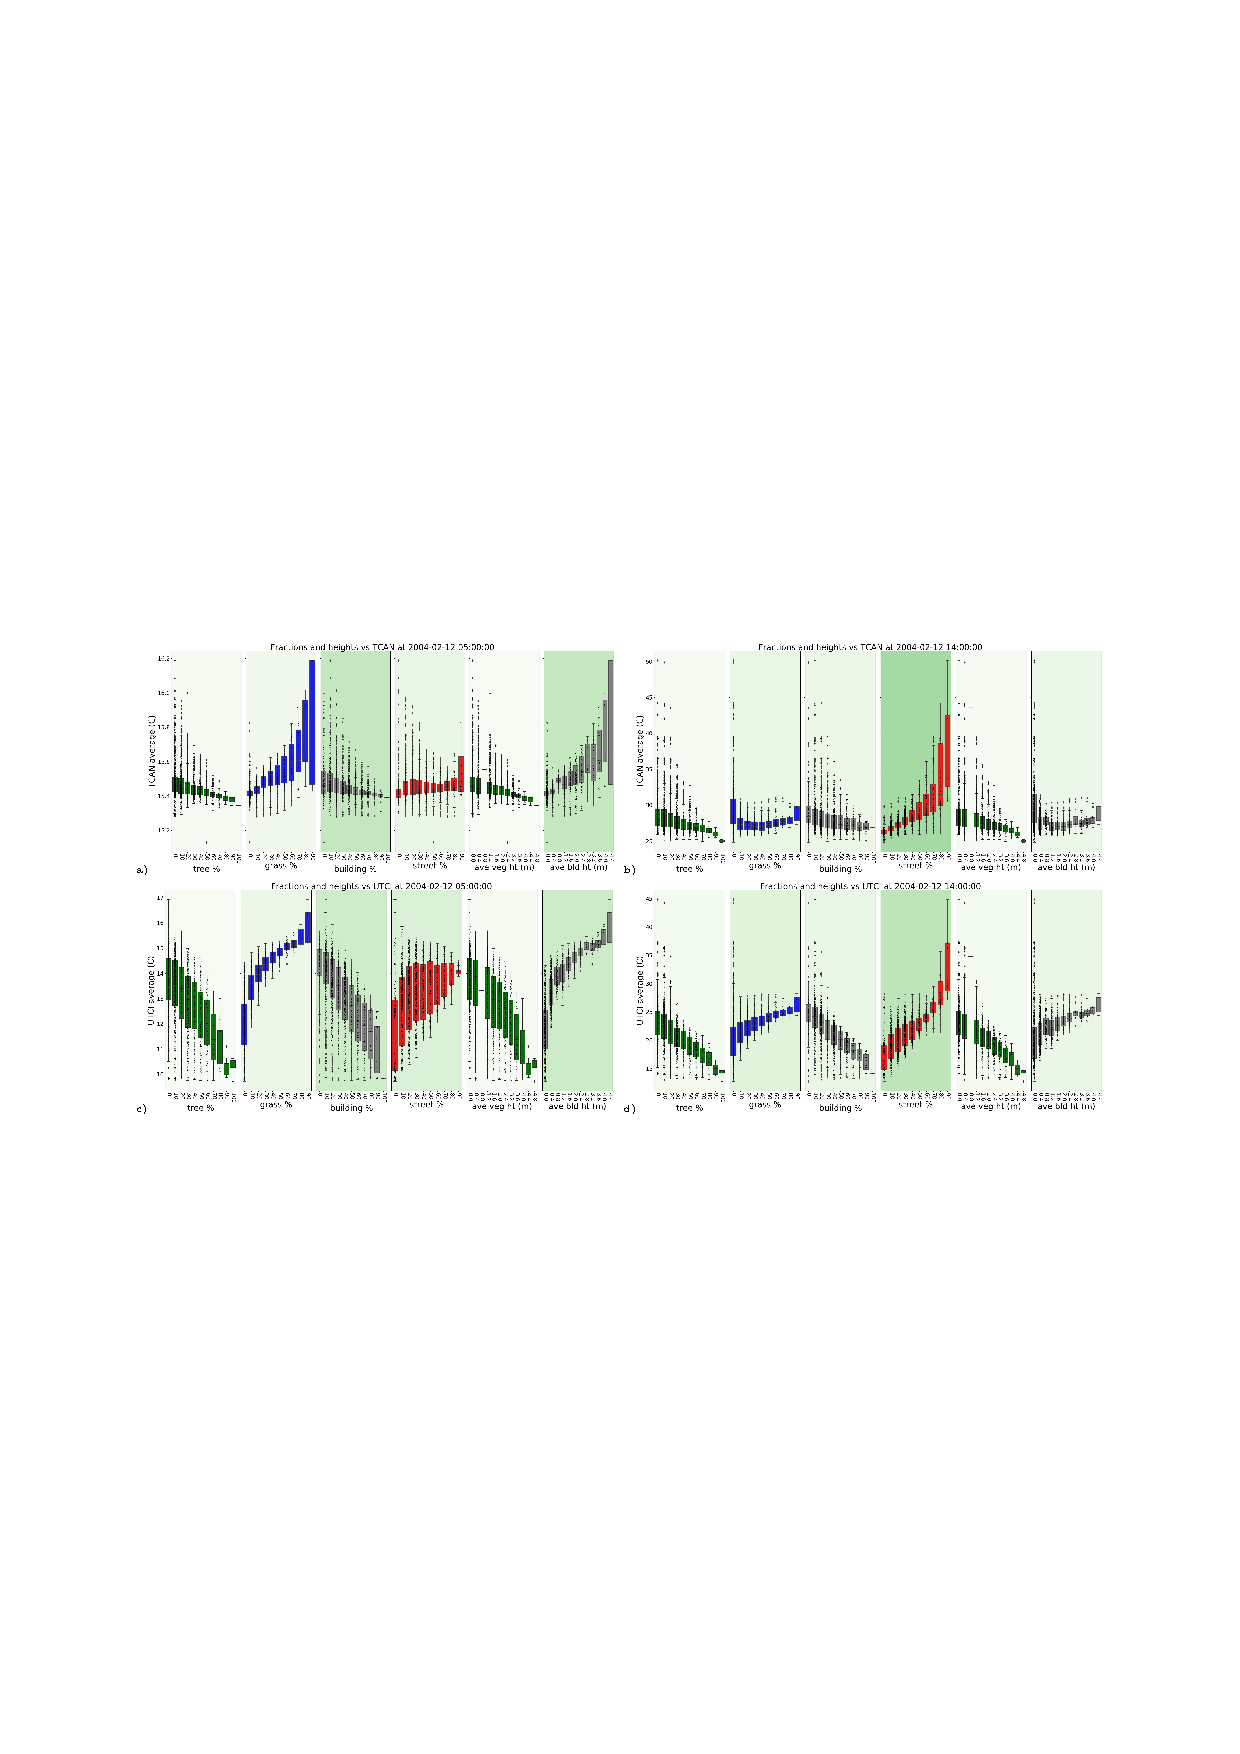
\includegraphics[page=1,trim={80 90 80 90},clip,width=\linewidth,
  height=\textheight]{Figures/Figures6.pdf}
\caption{\bf Surface fraction\remove{percentages} (trees, grass, buildings, and streets) and average height (vegetation and building) \remove{vs. }\add{clusters for 9814 scenario's} \gls{tcan} and \gls{utci} for February 12, 2004, 5am and 2pm. \add{\gls{tcan} is a single canyon averaged air temperature while \gls{utci} is a calculated mean at ground level.} The clusters will contain fractions up to the fractional or height breakpoint (i.e. 20\% includes the range 10 to 20\%  while 1.6m includes 1.2 to 1.6m). Feature importance for each temperature type is indicated by the green background tinting.}
 \label{fig:box5a} \label{fig:box14a}
\end{figure*} 


\begin{table}
\centering
\caption{\label{tab:tempDiffs}Maximum differences ($^{\circ}$C) in \gls{tcan} and \gls{utci} when increasing fractions from 10\% to 90\% and average vegetation and building heights to 4.4m. Bold indicates temperatures increase as fractions or heights increase. From maximum difference annotations in Figures \ref{fig:tcanday} and \ref{fig:utciday}}
\begin{tabular}{l l l l l l l l }
\hline
Temperature & Time & 
	$\uparrow$ Trees & 
	$\uparrow$ Grass & 
	$\uparrow$ Bld &
	$\uparrow$ Street &
	$\uparrow$ Veg Ht & 				
	$\uparrow$ Bld Ht 						
	\\
\hline
\gls{tcan} & Night &   
\textbf{0.2}&       %tree
-0.3& 				%grass
\textbf{0.6}&       %bld
\textbf{1.2} &       %street
\textbf{0.2}&       %veght
\textbf{0.5}		%bldht
\\
\gls{tcan} & Day &
-6.6&    	    %tree
-4.8&           %grass
\textbf{2.1}&   %bld
\textbf{14.5}&	%street
-6.8&    	 	%veght
\textbf{2.3}   %bldht
\\
\gls{utci} & Night &   
-5.8&         %tree
-5.7&         %grass
\textbf{3.8}& %bld
\textbf{3.3}&  %street
-5.6&         %veght
\textbf{4.0}   %bldht 
\\
\gls{utci} & Day &	
-7.9&           %tree
-9.6&           %grass
\textbf{5.5}&   %bld
\textbf{19.3}&   %street
-8.5&           %veght
\textbf{5.5}  %bldht
\\
\end{tabular}
\end{table}

Highlighted results are summarised in Table \ref{tab:tempDiffs}, taken from maximum difference annotations in Figures \ref{fig:tcanday} and \ref{fig:utciday}. Analysis of feature importance shows that building fractions and building heights are most significant for \gls{tcan} (Figure \ref{fig:featimpttcan}a) at night while building fractions and building heights are slightly more important than grass and streets and trees and vegetation heights are of the lowest importance for \gls{utci} (Figure  \ref{fig:featimptutci}b). During the daytime, street fractions are of the highest importance for both \gls{tcan} and \gls{utci}.

\begin{figure*}
\centering
{\tiny a)}\includegraphics[page=16,trim={55 270 40 270},clip,scale=0.45]{Figures/Figures6.pdf}
{\tiny b)}\includegraphics[page=17,trim={55 270 40 270},clip,scale=0.45]{Figures/Figures6.pdf}\\
\caption{\bf Feature importance in a) \gls{tcan} and b) \gls{utci} for the four surface fractions of streets, buildings, trees, and grass and average heights of vegetation and buildings across February 12, 2004.}
\label{fig:featimpttcan}
\label{fig:featimptutci}
\end{figure*}

\subsection{Distributions of temperatures across a diurnal cycle}\label{sec:resultsdist}

The preceding results (Section \ref{sec:resulttrends}) describe domain averaged ground level \gls{utci}, however each domain may contain a wide range of \gls{utci} values depending on micro-climate conditions. Therefore Figure \ref{fig:dist1} shows the intra-domain \gls{utci} distributions for select scenarios for each hour of February 12, 2004.\remove{Figure fig:dist1 shows the utci distributions for a number of selected scenarios across the 24 hours of February 12, 2004. The preceding results (Section sec:resulttrends) are based on mean values, averaged across the ground level results across each domain. However, different mixes of surface fractions and average heights result in widely varying distributions of temperatures (all in $^{\circ}$C).}

\begin{figure}    
\captionsetup[subfigure]{labelformat=empty}    
\centering    
\subfloat[a)]{\includegraphics[page=4,trim={60 225 40 265},clip,scale=0.55]{Figures/Figures6.pdf} }
\subfloat[b)]{\includegraphics[page=6,trim={150 225 40 265},clip,scale=0.55]{Figures/Figures6.pdf} }
\\
\subfloat[c)]{\includegraphics[page=9,trim={60 225 40 265},clip,scale=0.55]{Figures/Figures6.pdf} }
\subfloat[d)]{\includegraphics[page=10,trim={150 225 40 265},clip,scale=0.55]{Figures/Figures6.pdf}  }
\caption{\bf Distribution of \gls{utci} across February 12, 2004 for scenarios a) 50\% grass, 49.99\% trees, 0.01\% road, 0\% building, average vegetation height of 4m, and average building height of 0m, b) 29\% grass, 69\% trees, 1\% road, 1\% building, average vegetation height of 0.5m, and average building height of 5m, c) 40\% grass, 10\% trees, 20\% road, 30\% building, average vegetation height of 2m, and average building height of 14m, and d) 19\% grass, 20\% trees, 21\% road, 40\% building, average vegetation height of 1m, and average building height of 9m. Insert shows percent fractions of surface types. Hourly medians are annotated in red and hourly means in black. } \label{fig:dist1}
\end{figure} 


Figure \ref{fig:dist1}a presents a scenario with very low fractions of roads and buildings and as a result shows \gls{utci} temperatures mostly clustered in the lower ranges across day and night and very few locations that exceed the mid 20s during the day. Figure \ref{fig:dist1}b shows a scenario with a moderate amount of streets and buildings (20\% and 30\%) and moderate building heights, but yields similar results to Figure \ref{fig:dist1}a. Figure \ref{fig:dist1}d, with higher amounts of buildings and roads, shows a strong shift towards predominately hotter \gls{utci} temperatures (30$^{\circ}$C) across the entire domain during the daytime (also reflected in the median), while Figure \ref{fig:dist1}c, with slightly higher fractions of vegetation, shows a similar distribution but the median is much lower (in the lower 20s$^{\circ}$C).


These four example distributions show that urban heat has high variability at a micro-scale, even between scenarios with similar urban form and surface fractions. Mean temperature values (such as Table \ref{tab:tempDiffs}) can show general trends but each of these four distributions will contribute to four very different spatial experiences of urban heat and human thermal stress in each \remove{area}\add{domain}.


\section{Discussion}\label{sec:discussion}

\subsection{The influence of urban surfaces on urban heat}\label{sec:discinfluence}
Studies providing a systematic examination of the influence of varying surface fractions and urban heights are rare and generally based on remote sensing data. In this study, through systematic micro-climate modelling of a comprehensive range of surface fractions and average heights, the importance and relative influence of each feature type on the temperature types of \gls{tcan} and \gls{utci} was examined. For \gls{tcan}, at night-time, a narrow range of temperature variations were found, of approximately 1.0\SI{}{\degreeCelsius}. \add{Wind speed on February 12th (Figure \ref{fig:forcing}) was approximately 2m/s until the early afternoon, rising to approximately 6m/s, then dropping to 4 m/s after sunset. These higher wind speeds in the afternoon and evening had the effect of reducing the range of temperature variations in the evening and night compared to \cite{Stewart2021} where forcing wind speed was set to a constant 2.5m/s and resulted in wider ranges of night-time temperatures.} 

\add{In the presence of high wind speed at night,} increasing fractions of trees had a limited impact at midnight and contributed to a very slight increase (+0.2\SI{}{\degreeCelsius}) at dawn. Increasing building heights had a warming impact (+1.2\SI{}{\degreeCelsius}) while grass drove a slight cooling (-0.3\SI{}{\degreeCelsius}). Increasing street fractions contributed to a warming effect (+0.3\SI{}{\degreeCelsius}) at dawn. Building fractions and building heights were found to be the most significant features at night-time. During the daytime, the most important feature was the fraction of streets. Street fractions of 80 and 90\% can drive \gls{tcan} increases of up to 10 and 15\SI{}{\degreeCelsius} respectively while reductions are seen of about -5\SI{}{\degreeCelsius} when increasing grass and tree fractions from 0 to 100\%. 

\add{Some ground level LCZ based studies can provide some comparisons with our results. \cite{Holmer2013} finds that large vegetated sites cool quickly (have a large cooling rate) for 1-2 hours after sunset then cooling rates reduce and align with those of sparely vegetated sites for the rest of the night. We find that in air temperature, areas with high building heights and building fractions cools rapidly after sunset where in terms of \gls{utci}, areas with large trees and tree fractions cool most rapidly. In air temperatures differences observed across a year, \cite{Yang2018} finds LCZD (irrigated agriculture) is the coolest class in Nanjing, China while variations of LCZ2 (compact mid-rise but with different amounts of tree cover) are 2-3\SI{}{\degreeCelsius} warmer (those in the lower range have higher amounts of trees), LCZ4 (open high-rise) and LCZ8 (large low-rise) are 1.6 and 1.8\SI{}{\degreeCelsius} warmer respectively, and LCZ10 (heavy industry) is 2.7\SI{}{\degreeCelsius} warmer. These are generally in line with our findings. LCZ10 is mostly low rise and highly imperious and similar to our high street fraction scenarios which were substantially hotter than most other urban arrangements. Increasing fractions of trees had a moderating effect across all the scenarios. Finally, \cite{Puliafito2013} in comparing average air temperatures and Physiologically Equivalent Temperatures (PET) across transits of different LCZs to the mean of all their observations find the largest air temperature reductions of approximately 2\SI{}{\degreeCelsius} in the mornings and evenings in LCZD (0.6\SI{}{\degreeCelsius} in the afternoon), up to 1\SI{}{\degreeCelsius} reductions in the evening for LCZ3A (residential/dense trees) and LCZA (parks). Increases in air temperatures are observed of 1.5, 1.1, and 0\SI{}{\degreeCelsius} in downtown areas with scattered trees, medium trees, and high trees respectively. Trends in thermal comfort, PET, are similar but with larger magnitudes (i.e. -3.5\SI{}{\degreeCelsius} in LCZA), but at mid-day in the three downtown areas with varying tree cover the respective differences are 3.4, -0.2, and -5.3\SI{}{\degreeCelsius} PET. Vegetated areas have the largest air temperature reductions with the amount of tree cover a major factor in the magnitudes, while the differing thermal comfort benefits were strongly driven by amounts and heights of trees, but only at mid-day.}

Other studies show similar findings, often they were only able to demonstrate temperature trends rather than more detailed relationships. \cite{Emery2021}, in their observations of the influence of different \gls{lcz} classes on air temperature, found that the \gls{lcz} classes with the warmest air temperatures were those dominated by artificial, mineral, and impervious surfaces, while \gls{lcz} classes with vegetation were the coolest. However, they were not able to quantify the ranges of temperatures in more detail resulting from the different classes. Using remotely sensed \gls{lst}, \cite{Alexander2021} classified areas in a number of Danish cities into two classes of buildings and vegetation (essentially impervious vs. pervious) and into ranges of vegetation and building heights and examined their influence on \gls{lst}. He found \gls{lst} reduced by approximately 4\SI{}{\degreeCelsius} when vegetation fractions increased from 0-5 to 95-100\% and increased by 4\SI{}{\degreeCelsius} when building fractions increased by the same. Also, vegetation height had negative correlation with \gls{lst} but vegetation cover was found to be a stronger predictor. Building height had a positive correlation with \gls{lst}, but only up to 9m, and was not always found to have a strong influence on \gls{lst} in some of the studied cities. 

\cite{Peng2022} found, using a Random Forest regression of MODIS \gls{lst} observations of a highly urbanised city in Japan, the feature importance to predict urban heat island intensity in the daytime was highest for building density followed by distance to green space while at night-time distance to green space was the most important followed by distance to water and road density. In another study, using Landsat derived \gls{lst} of different \gls{lcz} classes across four African cities \citep{Li2022}, the highest \gls{lst} temperatures were found in the urban typologies of compact mid-rise, compact low-rise, and large low-rise (LCZ2, 3, and 8) and lowest in dense trees and water (LCZA and G). They found statistically significant differences between the LCZs, but not always when comparing \gls{lcz} classes in different cities of different K\"{o}ppen climate classifications, where often compact midrise (LCZ2) and open midrise (LCZ5) typologies were coolest (due to higher building heights). The \gls{lcz} typologies were found to be useful across single cities but could not always reliably be used to compare \gls{lcz} classes across different cities, especially those with differing climates.

While these results are able to show broad trends due to differing amounts of surface fractions, \remove{they cannot entirely predict the influences on}\add{linking \gls{lst} temperatures to} thermal comfort at\remove{the} ground \remove{level,}\add{level can be challenging and potentially misleading \citep{Coutts2016d,Stewart2021} as surface temperatures} underneath the urban canopy \remove{where surface temperatures}are moderated by shading from vegetation and \remove{buildings.}\add{buildings \citep{Coutts2015,Lee2018,Krayenhoff2021}.} This is a limitation of remotely sensed \gls{lst} observations, that can only provide the temperatures at the top of the urban canopy. Some studies are able to provide some additional data on the under canopy impacts through observations. For example, micro-climate observations from \cite{Broadbent2017a} showed that in a residential suburb, \gls{tsfc} temperatures of concrete, buildings, and bare ground were 2.4, 3.1, and 1.1\SI{}{\degreeCelsius} hotter than the area averages during the day and areas with trees, irrigated grass, and low vegetation were 3.0, 7.7, and 6.8\SI{}{\degreeCelsius} cooler. While high resolution spatial air temperature are difficult to observe, \cite{Broadbent2017a} also found increases over the suburb average in air temperature of 1\SI{}{\degreeCelsius} in the cluster type of urban mid-rise and 0.5\SI{}{\degreeCelsius} with the type urban residential. They also found an irrigated grass daytime cooling effect of -0.1\SI{}{\degreeCelsius} per 5\% fraction increase. \cite{Middel2019a} found trees could provide large reductions in \gls{tmrt} on extreme heat days, with reductions up to 33.4\SI{}{\degreeCelsius} and with sky view factor (SVF) highly influential in determining the reductions, 4\SI{}{\degreeCelsius} \gls{tmrt} reductions per 0.1 SVF decreases. However, the trade-offs are a warming effect at night of up to 5\SI{}{\degreeCelsius}. In addition, they found replacing impervious with pervious surfaces can decrease \gls{tmrt} by 1.0-1.5\SI{}{\degreeCelsius} per tenth of land converted and unshaded irrigated grass could reduce \gls{tmrt} by more than 10\SI{}{\degreeCelsius} compared to impervious surfaces with unirrigated grass providing still about half as much in reductions. Additionally, \cite{Krayenhoff2021} finds that trees provide additional 0.3\SI{}{\degreeCelsius} reductions per 0.10 canopy cover increase.

\add{The results reported in the studies compared above of trends and relationships between different urban forms and observed temperature outcomes (both air temperatures and thermal comfort indexes) demonstrates the difficulty in designing and testing mitigation measures that are based on changing individual design parameters once at time. Quantifying the impact of the measures, when in reality each urban change is interdependent on other elements of urban form and moderate the impacts (often in a non-linear fashion), make quantifying their impacts difficult. This is especially true when the additional complexity of regional geography and human activity is added into the mix. This points to the necessity of a modelling approach that can examine a comprehensive range of representative combinations of urban form at once and in isolation from as many other compounding interdependencies to overcome the difficulties in attributing the influence of each individual urban element and allow a generalisation of the findings to other scenarios and cities.}

\subsection{City scale heat maps from micro-climate modelled results}\label{sec:resultsheatmaps}

Following on from the results of the comprehensive urban form analysis and reflecting many of the specific findings of other studies of the impact of differing types of urban form on urban heat, the modelled results underlying this analysis were applied to demonstrate their application to a city-wide heat mapping exercise. These heat maps show the impact of present day urban form across a number of Australian cities, isolated from geography, topography, and local weather conditions. \add{Surface fractions and average building and vegetation heights for Melbourne and Sydney were calculated for 100$\times$100m locations using 2 meter resolution land cover and building and tree footprints and heights from Geoscape \citep{Geoscape2020}.} Figure \ref{fig:TaMelb} shows city-wide heat maps of \gls{tcan} and \gls{utci} in Melbourne at 2pm on February 12, 2004 constructed by matching the closest matching parameters for each locations from the 9814 modelled scenario results. A narrow range of air temperatures are seen across most of the city, closely aligned to the modelling forcing temperature at 2pm of 25.9\SI{}{\degreeCelsius}. Higher temperatures can be seen in areas corresponding to higher fractions of roads and to a lesser degree of buildings. No particular reductions of air temperatures are seen in areas corresponding to higher levels of trees or grass surface fractions. Fractional breakdowns of surfaces types across Melbourne are shown in Supplementary Figure \ref{fig:melfracs}. 


\begin{figure*}
\centering
a)\includegraphics[page=18,trim={63 421.25 370 215},clip,scale=1.3]{Figures/Figures6.pdf}
b)\includegraphics[page=18,trim={234 220 195 420},clip,scale=1.3]{Figures/Figures6.pdf}
\caption{\bf a) \gls{tcan} and b) \gls{utci} heatmaps on February 12, 2004 at 2pm generated by matching the closest matching parameters of surface fractions and average heights for each 100$\times$100m location in Melbourne from 9814 modelled scenario results (in \SI{}{\degreeCelsius}). }
 \label{fig:TaMelb}  \label{fig:utciMelb}
\end{figure*}


Wider ranges of surface temperatures are seen across Melbourne. Some slight reductions of surface temperatures (below the forcing air temperature) are seen in areas that correspond to higher fractions of grass and of trees. However, strong increases in surface temperatures \add{are seen} in areas with higher fractions of street surfaces, even in areas with street fractions as low as 30\%. Very strong increases in surface temperatures can be seen in areas with high street surface fractions, for example Melbourne Airport in the north west, the central business district (CBD) in the city centre, and Moorabbin Airport in the city south east.

Figure \ref{fig:Melb_TSFC12_85} presents a comparison of modelled \gls{tsfc} to Landsat 8 \gls{lst} data. Figure \ref{fig:Melb_TSFC12_85}a shows Landsat 8 imagery captured on a cloudless day that mostly closely corresponds to the modelled conditions, 10am December 11, 2018 when local conditions of air temperature on this day were minimum and maximum of 22 and 26\SI{}{\degreeCelsius}. Figure \ref{fig:Melb_TSFC12_85}b shows \gls{tsfc} created from modelled results at 10am on February 12, 2004 and February 14, 2004. 

In comparing the constructed \gls{tsfc} heat maps with the LST imagery, some observations can be made. However note, the two datasets measure different things and might not be entirely comparable. \gls{lst} observations are captured by satellite and correspond to temperatures at the top of the urban canopy (i.e. the tops of trees and buildings) while the modelled \gls{tsfc} corresponds to ground surface temperatures and will generally be cooler as they include areas that are shaded by tree canopies and buildings. In addition, \gls{lst} observations are influenced by additional factors than just the urban form including topography and localised weather conditions. In Figure \ref{fig:Melb_TSFC12_85}a, the cooler locations in the \gls{lst} observations mostly include locations immediately off the coast and in the eastern fringes of Melbourne, the Dandenong Ranges which range from 500m to over 1000m in elevation, while the majority of central and inner Melbourne is under 100m in elevation. The main differences between the \gls{lst} observations and the modelled results are strongly related to the surface fraction types, which a strong correlation between the differences and building and street fractions and a strong negative correlation with grass surface fractions. 

\begin{figure*}
\centering
a)\includegraphics[page=13,trim={75 225 195 245},clip,scale=0.54]{Figures/Figures6.pdf}
b)\includegraphics[page=11,trim={63 230 210 250},clip,scale=0.56]{Figures/Figures6.pdf}
\caption{\bf a) Landsat 8 land surface temperature (\SI{}{\degreeCelsius}) captured 10am December 11, 2018. Local conditions of air temperature on this day were minimum and maximum of 22 and 26\SI{}{\degreeCelsius}. b) Modelled \gls{tsfc} (\SI{}{\degreeCelsius}) on February 12, 2004 at 10am generated by matching the closest matching parameters of surface fractions and average heights for each 100$\times$100m location in Melbourne from 9814 modelled scenario results.}
 \label{fig:Melb_TSFC12_85}
\end{figure*}


Additionally, heat maps were generated for other cities. Using the 9814 modelled scenario results, heat maps of \gls{tcan} and \gls{utci} (Supplementary Figure \ref{fig:TaSyd}) were created for Sydney for February 12, 2004 at 2pm by matching the closest matching parameters, as calculated from Supplementary Figure \ref{fig:sydfracs}, for each location. Supplementary Figure \ref{fig:Sydney-Landsat-LST-11-03-2019}a shows cloudless Landsat 8 observations from 10am March 11, 2019 (local conditions of air temperature on this day were minimum and maximum of 22 and 26\SI{}{\degreeCelsius}) while Supplementary Figure \ref{fig:TaSyd}b shows \gls{tsfc} heatmaps created from modelled results at 10am on February 12, 2004. 

The results are similar to those from Melbourne. Ranges of \gls{tcan} are generally very narrow with small localised hot spots. The \gls{lst} observations reflect a different topography than Melbourne with a larger influence of coastal features and a smaller range of elevations. Much of the central city is under 100m \add{elevation} and only approaching 200m in the north east areas. The areas with higher ranges of \gls{lst} are concentrated in the \remove{agricultural}western regions of the city (with very high percentages of grass/low vegetation land cover fractions). Similar to Melbourne, \remove{correlations between differences between}\gls{lst} and \gls{tsfc} are strongly negatively correlated with grass fractions but somewhat less correlated with building and street fractions.

\add{This study demonstrates a new method of massive ensemble modelling, to efficiently perform city scale modelling at a micro-scale to isolate the impacts of the urban form and fabric on urban heat. The overall method can be replicated with any suitable micro-climate scaled model (or with improved versions of VTUF-3D). Future work has been planned to address two potential limitations of this study: model bias and expanding the range of representative weather conditions. VTUF-3D has been extensively evaluated using the forcing data used in this study, but like all models, has biases. VTUF-3D might underestimate surface temperatures of grass. Analysis of correlations between the surface fractions and differences between observed \gls{lst} and modelled \gls{tsfc} suggest that the temperature trends for streets (correlations of 0.69 and 0.72 in Melbourne respectively) and buildings (0.78 and 0.72 in Melbourne) are reasonable but the magnitude is too high while grass (-0.80 and -0.85) trends are also reasonable but too low. Meanwhile the correlations for trees are very low suggesting the variations are not regular. As the percent fractions for trees just means that tree cover exists, it does not fully characterise the tree cover, such as the level of canopy cover (i.e. a leaf area index) or the variations in coverage amounts. VTUF-3D is undergoing continuous improvement, especially its vegetation scheme, and future research will apply these improvements to similar assessments. A second limitation planned to be addressed with further research is to ensure the method models a full set of representative days and weather types for a city. For this, weather clustering \citep{Shobha2017,Acero2019,nazarian2019outdoor} will be utilised to generate forcing data for the full range of weather condition types experienced in cities and allow the analysis of thermal comfort across the range of extreme heat days to warm down to extreme cold winter days.}


\section{Conclusion}\label{sec:conclusion}

Observational studies have previously attempted to quantify the influence of urban form on urban heat largely using two different types of observations,\remove{top of the urban canopy} remotely sensed \gls{lst} and under the urban canopy ground level micro-scaled observations. \add{Satellite or aerial remote sensing observes only sky-facing surfaces (e.g. roofs and the vegetation canopy).} Micro-scaled ground based observations can provide detailed assessments under the canopy, but are time-intensive, requiring substantial effort to collect, and are difficult to scale up to a city-wide scale. \remove{The observations from other studies demonstrate the usefulness of the results and the application of the systematic modelling in this study.}The observations \add{reported in these studies} show many of the trends found in this study, including the large increases in both \gls{tcan} and \gls{utci} with increasing road fractions, as well as decreases of both temperature types during the daytime with increasing vegetation fractions and heights. Our method also overcomes difficulties encountered with the LCZ-based observations and modelling assessments, where the highly urbanised classes were found to be hotter while the natural classes were cooler, findings in line with our results. However, due to the broad \remove{ranges}\add{range of possible morphology within} each LCZ \remove{can represent}along with the (often non-linear) interactions between the parameters, detailed \remove{and specific quantifications have}\add{quantification has} not always been possible in the studies utilising LCZs (i.e. \cite{Emery2021}).\remove{Our method allows the influence of elements of urban form to be quantified as heights and fractional amounts of land cover are incrementally increased and decreased.}


Using the comprehensive urban form analysis methods in this study allows a determination of the importance and relative influence of each surface type and feature height on thermal performance (e.g. increasing street fractions from 50\% to 80\% can drive air temperature increases of up to 5\SI{}{\degreeCelsius}). Additionally, once these relationships have been quantified, it becomes possible to apply the results across a broad area, a city-wide assessment of thermal comfort. This is an area of broad interest as evidenced by the numerous studies attempting this through satellite observed \gls{lst}. \remove{But the modelled approach eliminates the difficulty using top of the canopy lst observations to derive ground level temperatures, temperatures that also include the shading impacts of the urban canopy. More importantly,}\add{However, a comprehensive modelling approach is able to capture both sky-facing and pedestrian-level conditions at city scales. Additionally,} it removes geographic influences (such as topography, ocean effects, and local weather) from the results and allows an assessment based solely on the urban and natural forms of the urban areas. This allows \add{an assessment at city scales of problematic existing urban form, and allows} mitigation strategies to be tested based on the urban form elements that can be changed, while removed from influences that cannot be redesigned. \add{Heat can often be inequitably distributed \citep{Jenerette2018,Nazarian2021,Guardaro2022} where more challenging thermal conditions can be experienced in parts of urban areas with low levels of vegetation and canopy cover and high impervious surface fractions compared to leafy enclaves near large water bodies. Understanding the impacts of the urban form can help weigh the relative importance of urban interventions, providing local context to the anticipated impact of the intervention with the required urgency.}


\remove{In addition, the ability to capture at high temporal and spatial scales the high variability of elements of urban heat (i.e. the distributions of utci in different scenarios in Figure fig:dist1) point to new directions for future research. Urban areas can be characterised by the quality of their connectedness of cooling and how well each area supports pedestrians navigating urban arrangements to minimise their thermal stress.} \remove{In addition, future work can address one potential limitation of this study. VTUF-3D has been extensively evaluated using the forcing data used in this study, but like all models, has biases. Is is possible that VTUF-3D is underestimating temperatures of grass. The correlations between the surface fractions and differences between observed LST and modelled Tsfc suggest that the temperature trends for streets (0.69 and 0.72 in Melbourne) and buildings (0.78 and 0.72 in Melbourne) are reasonable but the magnitude is too high while grass (-0.80 and -0.85) trends are also reasonable but too low. Meanwhile the correlations for trees are very low suggesting the variations are not regular. As the percent fractions for trees just suggests that tree cover exists, it does not fully characterise the tree cover, such as the level of canopy cover (i.e. a leaf area index). VTUF-3D is undergoing continuous improvement, especially its vegetation scheme. The overall method in this study can be repeated using this or other improved micro-climate models in future work. }

\printglossaries

\section{References}\label{sec:ref}
\bibliographystyle{elsarticle-harv} 
\bibliography{BlockTypologies-EBP}

\newglossaryentry{utci}{name=$UTCI$,description={universal thermal climate index (\SI{}{\degreeCelsius})}}
\newglossaryentry{tsfc}{name=$T_{sfc}$,description={surface temperature (\SI{}{\degreeCelsius})}} 
\newglossaryentry{tcan}{name=$T_{can}$,description={canyon averaged air temperature (\SI{}{\degreeCelsius})}} 
\newglossaryentry{ta}{name=$T_{a}$,description={Air temperature (\SI{}{\degreeCelsius})}} 
\newglossaryentry{tmrt}{name=$T_{mrt}$,description={mean radiant temperature (\SI{}{\degreeCelsius})}} 
\newglossaryentry{lst}{name=$LST$,description={land surface temperature (\SI{}{\degreeCelsius})}}
\newglossaryentry{lcz}{name=LCZ,description={local climate zones}}
\newglossaryentry{htc}{name=HTC,description={human thermal comfort}}
\newglossaryentry{WUDAPT}{name=WUDAPT,description={World Urban Database and Access Portal Tools}}

\clearpage

\section{Acknowledgements}\label{sec:ack}
KAN is supported by NHMRC/UKRI grant (1194959).

%\section{Credit Author Statement}\label{sec:credit}
%
%\textbf{KAN}: Conceptualization, Methodology, Software, Formal Analysis, Writing - Original Draft, Writing - Review \& Editing, Visualization.
%\textbf{NN}: Methodology, Writing - Original Draft, Writing - Review \& Editing.
%\textbf{MJL}: Methodology, Writing - Review \& Editing.
%\textbf{MAH}: Methodology, Writing - Original Draft, Writing - Review \& Editing.
%\textbf{SS}: Methodology, Writing - Review \& Editing.
%\textbf{JT}: Writing - Review \& Editing.
%\textbf{MN}: Data Curation.
%\textbf{BG}: Writing - Review \& Editing.
%\textbf{MS}: Writing - Review \& Editing.




\section{Supplementary Figures}\label{sec:suppfig}
\beginsupplement


\begin{figure*}
\centering
\includegraphics[page=19,trim={55 215 200 215},clip,scale=1.0]{Figures/Figures6.pdf}
\caption{\bf Surface fractions (in percentages) of a) grass, b) trees, c) buildings, and d) streets across Melbourne.}
 \label{fig:melfracs}
\end{figure*}

\begin{figure*}
\centering
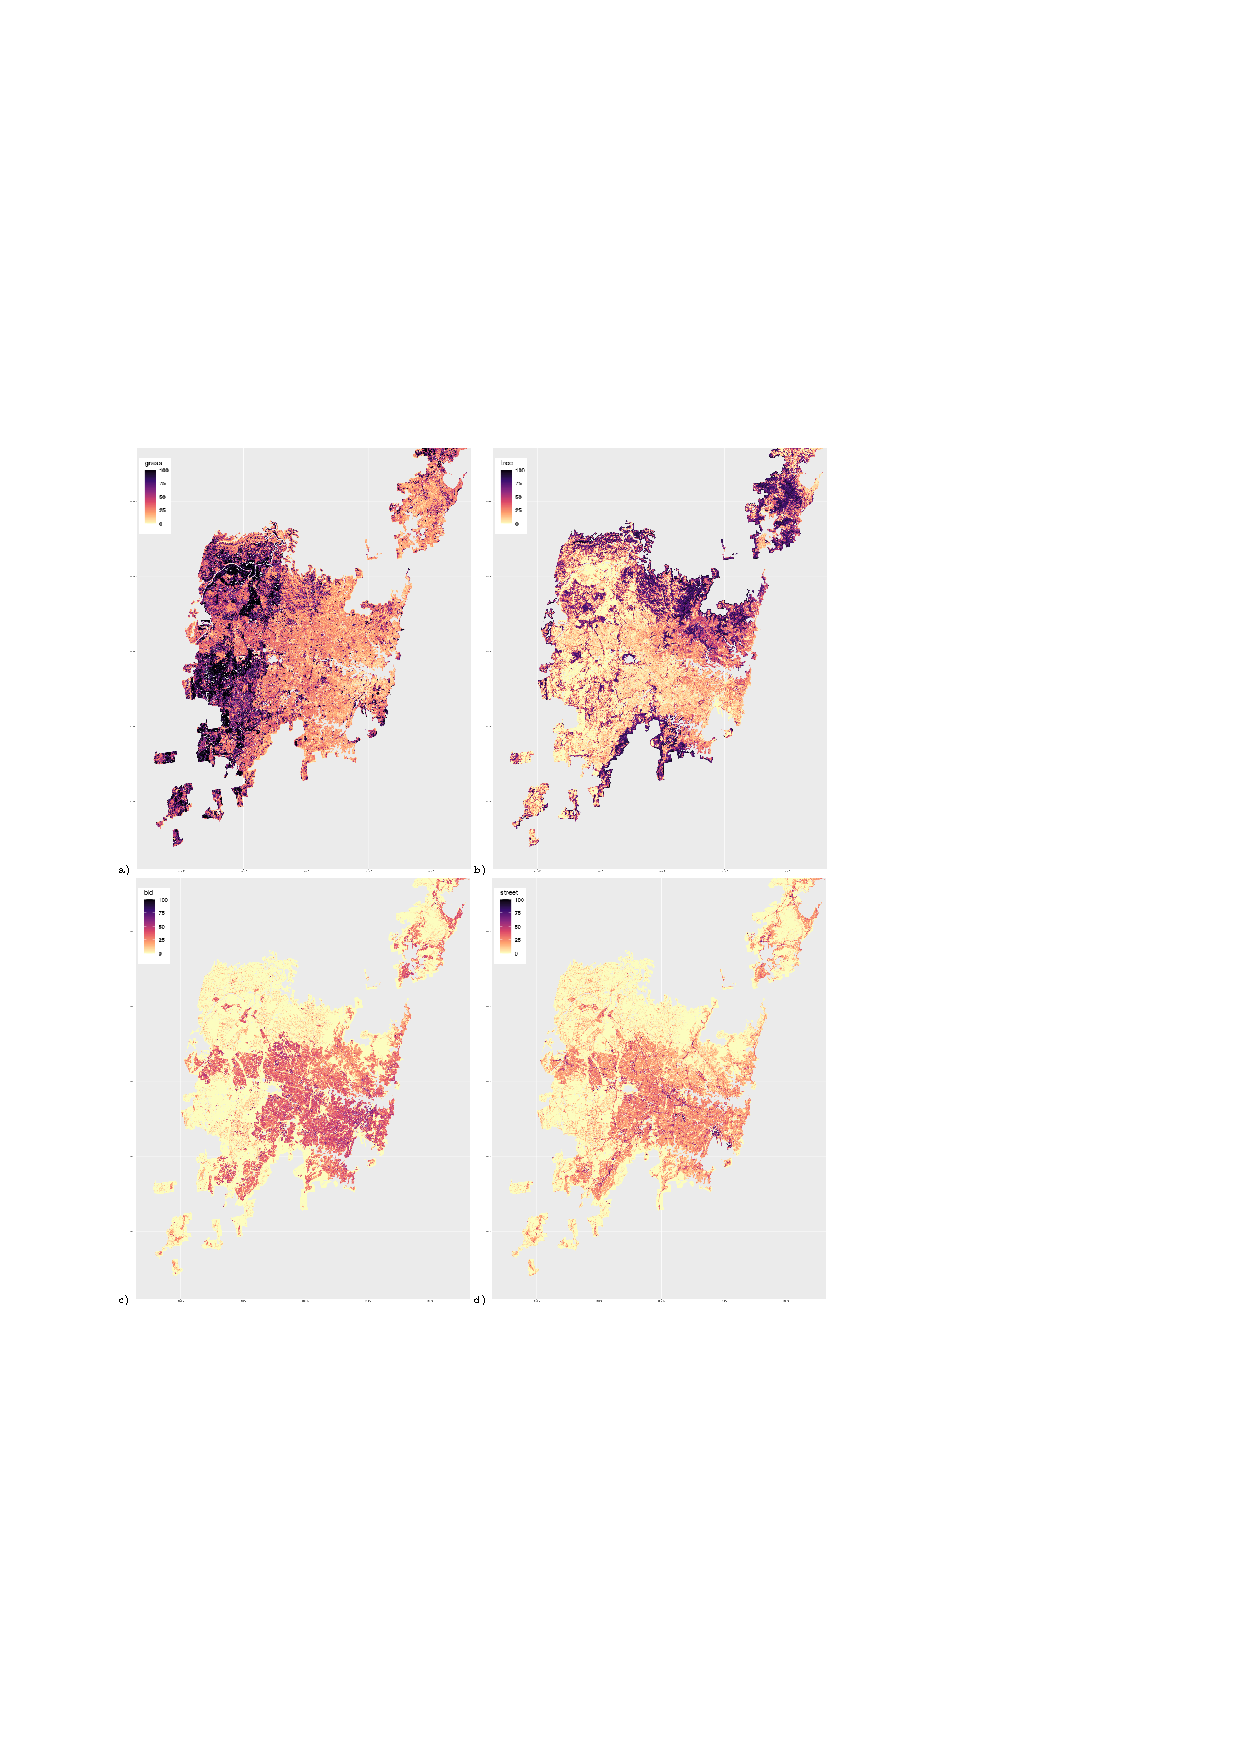
\includegraphics[page=1,trim={55 215 200 205},clip,scale=1.0]{Figures/Figures7.pdf}
\caption{\bf Surface fractions (in percentages) of a) grass, b) trees, c) buildings, and d) streets across Sydney.}
 \label{fig:sydfracs}
\end{figure*}

\begin{figure*}
\centering
a)\includegraphics[page=2,trim={63 421.25 370 215},clip,scale=1.3]{Figures/Figures7.pdf}
b)\includegraphics[page=2,trim={234 220 195 420},clip,scale=1.3]{Figures/Figures7.pdf}
\caption{\bf a) \gls{tcan} and b) \gls{utci} heatmaps on February 12, 2004 at 2pm generated by matching the closest matching parameters of surface fractions and average heights for each 100$\times$100m location in Sydney from 9814 modelled scenario results (in \SI{}{\degreeCelsius}).  }
 \label{fig:TaSyd} \label{fig:utciSyd}
\end{figure*}

%16 Sydney-Landsat-LST-11-03-2019  %//  11/03/2019	22	26
\begin{figure*} 
\centering
a)\includegraphics[page=14,trim={65 245 245 240},clip,scale=0.53]{Figures/Figures6.pdf}
b)\includegraphics[page=12,trim={60 220 210 225},clip,scale=0.48]{Figures/Figures6.pdf}
\caption{\bf a) Landsat 8 land surface temperature (\SI{}{\degreeCelsius}) captured 10am March 11, 2019. Local conditions of air temperature on this day were minimum and maximum of 22 and 26\SI{}{\degreeCelsius}. b) Modelled \gls{tsfc} (\SI{}{\degreeCelsius}) on February 12, 2004 at 10am generated by matching the closest matching parameters of surface fractions and average heights for each 100$\times$100m location in Sydney from 9814 modelled scenario results.}
 \label{fig:Sydney-Landsat-LST-11-03-2019}
 \label{fig:Sydney_TSFC12_85}
\end{figure*}


\begin{figure*}
\centering
\includegraphics[page=21,trim={175 300 180 300},clip,scale=1.0]{Figures/Figures6.pdf}
\caption{\bf Distribution of surface types across all modelled scenarios.}
 \label{fig:surfdist}
\end{figure*}



\end{document}
